\documentclass[a4paper,11pt]{article}
\usepackage[T1]{fontenc}
\usepackage[utf8]{inputenc}
\usepackage[french]{babel}
\usepackage[margin=2cm]{geometry}
\usepackage{lmodern,microtype,graphicx,booktabs,tabularx,array,enumitem,caption,needspace}
\usepackage{titlesec}
\titlespacing*{\section}{0pt}{10pt}{6pt}
\titlespacing*{\subsection}{0pt}{9pt}{4pt}
\usepackage[hidelinks]{hyperref}
\setlength{\parindent}{0pt}
\setlength{\parskip}{4pt}
\setlist[itemize]{nosep,leftmargin=1.4em,topsep=3pt}
\captionsetup{font=small,labelfont=bf,skip=4pt}
\renewcommand{\arraystretch}{1.15}
\newcolumntype{Y}{>{\raggedright\arraybackslash}X}
\setlength{\emergencystretch}{2em}
\begin{document}
\noindent
\includegraphics[width=4.5cm]{images/polytech-marseille.pdf}\hfill
\includegraphics[height=1.3cm]{images/amu.pdf}\par
\vspace{2pt}
\begin{center}
{\LARGE\bfseries Intern}\par
\vspace{3pt}Compte rendu du projet de virtualisation -- Polytech\par
Omar Benjelloun -- Hicham Mohammed\par
{\small Dépôt et livrables : \url{https://github.com/OmarBenje/Intern}}
\end{center}
\vspace{3pt}
\subsection*{Résumé}
Nous avons déployé Intern, notre application React, Django et PostgreSQL, sur trois VM VirtualBox puis trois conteneurs Docker. Nous avons comparé leur consommation au repos et leur comportement sous charge avec JMeter.

Docker utilise moins de mémoire et de disque, mais démarre plus lentement dans notre configuration rootless avec FUSE. Les mesures présentées dans ce rapport montrent l'importance des réglages choisis.

\section{Contexte et objectifs}
L'objectif du module était de construire une application en trois couches, puis de comparer deux types de virtualisation : les VM, chacune avec son propre noyau, et les conteneurs, qui partagent celui de l'hôte. Nous avons suivi les quatre parties du sujet : développement (étapes 1 à 6), VM (7 à 10), Docker (11 à 14) et tests de charge (15 à 18).

Nous avons adapté le sujet à Intern. Un candidat peut y chercher un stage, gérer son profil et son CV, puis suivre ses candidatures. Un recruteur peut publier des offres et consulter les candidatures reçues. Nous avons gardé le même code dans les deux déploiements pour pouvoir comparer leur comportement.

\subsection{Architecture en trois couches}
\begin{center}\begin{minipage}{\linewidth}\small
\captionof{table}{Rôle des composants de l'application.}\label{tab:1}
\begin{tabularx}{\linewidth}{YYY}
\toprule
\textbf{Couche} & \textbf{Technologie} & \textbf{Rôle} \\
\midrule
Présentation / proxy & Nginx, client React & Seul point d'entrée ; sert le client et les fichiers statiques, transmet /api au métier \\
Métier & Python 3.12, Django, Django REST Framework, Gunicorn & API, sessions, règles d'accès, validation \\
Données & PostgreSQL 16 & Persistance, contraintes d'intégrité, recherche textuelle \\
Fichiers & Cloudflare R2 (bucket privé, région UE) & CV, lettres et pièces des candidatures \\
\bottomrule
\end{tabularx}
\end{minipage}\end{center}
La figure~\ref{fig:1} résume les échanges entre les composants du tableau~\ref{tab:1}.

\begin{center}\begin{minipage}{\linewidth}\centering
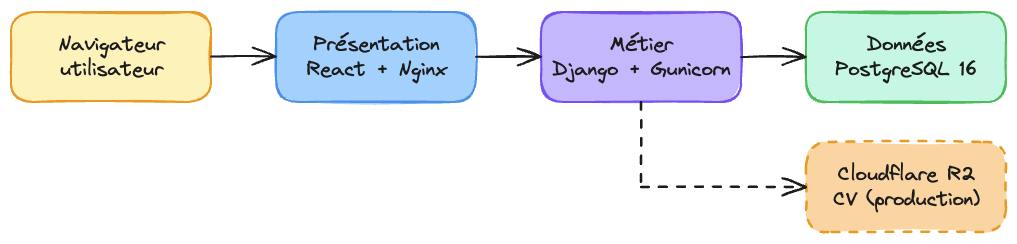
\includegraphics[width=.92\linewidth,height=4.4cm,keepaspectratio]{images/figure-1.png}
\captionof{figure}{Architecture générale d'Intern et stockage des documents.}\label{fig:1}
\end{minipage}\end{center}
\clearpage
\section{Conception de l'application}
\subsection{Analyse et prototype}
Avant de coder, nous avons défini les parcours des candidats, recruteurs et administrateurs, les règles d'accès et les principaux cas d'erreur. Le prototype interactif Figma nous a servi de repère pour construire l'interface.

Le document \href{https://github.com/OmarBenje/Intern/blob/master/docs/Figma.md}{\nolinkurl{docs/Figma.md}} relie le prototype, les étapes de conception, les corrections et les preuves. Les prompts Figma originaux ne sont plus disponibles. Quatre exemples reconstitués, explicitement signalés, illustrent les demandes et les corrections. Le prompt original de génération du visuel d'authentification est conservé séparément ; il concerne l'image décorative.

\subsection{Architecture de la base de données}
Nous avons regroupé le catalogue d'offres et les données privées dans une seule base PostgreSQL. Elle assure aussi la recherche textuelle grâce aux index GIN et garde une file de messages transactionnelle (outbox) pour les traitements en arrière-plan. Nous n'avons pas ajouté de base NoSQL ni de moteur vectoriel.

La base compte 72 tables au total, à partir de 34 modèles Django et des tables du framework. La figure~\ref{fig:2} présente les principales tables métier.

\begin{center}\begin{minipage}{\linewidth}\centering
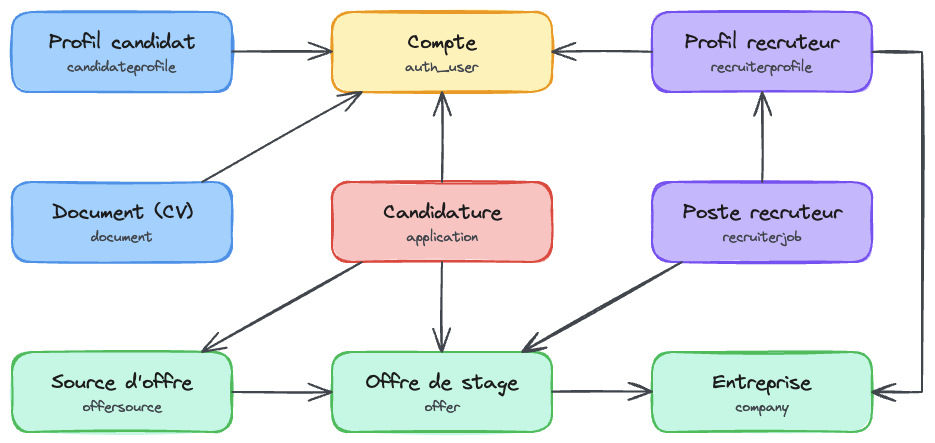
\includegraphics[width=.92\linewidth,height=5.3cm,keepaspectratio]{images/figure-2.png}
\captionof{figure}{Principales tables métier et leurs relations.}\label{fig:2}
\end{minipage}\end{center}
\clearpage
\subsection{Ingénierie front : du prototype à une interface fonctionnelle}
Le travail de présentation comprend les parcours, les états de l'interface et leur raccordement au métier. React et TypeScript organisent les écrans ; les composants partagés et les variables CSS de couleurs, d'espacement et de typographie rendent les évolutions cohérentes. Le client HTTP centralise les appels à l'API, les cookies de session, le CSRF et les erreurs réseau.

L'inscription illustre ce passage du prototype au produit : le formulaire conserve les saisies lors d'un retour, associe chaque erreur au champ concerné et désactive la soumission pendant la requête. Après création, il affiche l'attente d'activation renvoyée par Django. Les labels restent présents, les contrôles sont utilisables au clavier et les retours d'erreur ne reposent pas uniquement sur la couleur.

Les revues conservées retracent des améliorations concrètes : simplification de l'authentification, rapprochement de l'action de candidature et organisation du profil en sections avec brouillons indépendants. Les tests ciblés couvrent notamment les petits écrans, le zoom du texte, le contraste, le focus et la réduction des animations. Ils ne constituent pas un audit complet d'accessibilité.

La validation frontend consigne 104 tests navigateur réussis avec API contrôlée et 3 scénarios optionnels ignorés ; une recette séparée vérifie les parcours avec Django et PostgreSQL réels. Ces résultats sont ceux des vérifications archivées. Pour reprendre le travail, une équipe dispose du prototype, des sources React, des captures et des commandes de vérification dans le \href{https://github.com/OmarBenje/Intern/blob/master/docs/Figma.md}{document Figma} et la \href{https://github.com/OmarBenje/Intern/blob/master/frontend/VALIDATION.md}{validation du frontend}.

\subsection{Stockage des CV sur Cloudflare R2}
En production, les CV, lettres et pièces jointes sont conservés dans un bucket Cloudflare R2 privé, sous juridiction européenne. Django y accède avec boto3, via l'API compatible S3. PostgreSQL garde uniquement les références, métadonnées et empreintes SHA-256 des fichiers.

\begin{itemize}
\item Ce choix permet de recréer une VM ou un conteneur sans perdre les documents conservés sur R2.
\item Le bucket n'est pas public : Django vérifie les droits de l'utilisateur avant de lui renvoyer un fichier.
\item Chaque document est limité à 10 Mo ; son empreinte SHA-256 permet de contrôler son intégrité.
\item Le paramètre PRIVATE\_STORAGE\_BACKEND permet de choisir le stockage local privé pour le développement et les mesures, ou R2 en production, sans modifier le code.
\item Nous avons vérifié l'accès au bucket avec les identifiants de l'application et la présence des documents envoyés depuis Intern.
\end{itemize}
\subsection{Couche métier, interface et recette}
Django REST gère les sessions, la protection CSRF, le hachage scrypt et la limitation des tentatives de connexion. Les droits d'accès sont vérifiés à chaque requête. Nous avons rejoué les parcours du cahier de tests dans un navigateur sur les deux déploiements. La comparaison de l'application avec le prototype Figma a été réalisée (T25) ; son achèvement a été confirmé par l'équipe.

\clearpage
\section{Déploiement en machines virtuelles}
\subsection{Machines et réseau}
Hôte : Fedora Linux 42, Intel Core i5-1235U (12 processeurs logiques), 15,3 Gio de RAM, VirtualBox 7.2.8.

Nous avons créé trois clones d'Ubuntu Server 24.04.5 LTS, sans interface graphique, avec un snapshot \og base propre\fg{} avant chaque étape.

\begin{center}\begin{minipage}{\linewidth}\small
\captionof{table}{Ressources et accès réseau des VM.}\label{tab:2}
\begin{tabularx}{\linewidth}{YYYY}
\toprule
\textbf{VM} & \textbf{vCPU / RAM} & \textbf{Adresse interne} & \textbf{Accès extérieur} \\
\midrule
vm-proxy & 1 / 1 Gio & 10.10.10.10 & NAT ; seule redirection : hôte 127.0.0.1:8080 $\rightarrow$ 80 \\
vm-metier & 2 / 2 Gio & 10.10.10.20 & Aucun ; pas de route par défaut \\
vm-donnees & 2 / 2 Gio & 10.10.10.30 & Aucun ; pas de route par défaut \\
\bottomrule
\end{tabularx}
\end{minipage}\end{center}
Le tableau~\ref{tab:2} présente les trois VM. La figure~\ref{fig:3} montre leur réseau interne intnet-app (10.10.10.0/24). Nous avons fixé les adresses avec Netplan et identifié les interfaces par leur adresse MAC.

\begin{center}\begin{minipage}{\linewidth}\centering
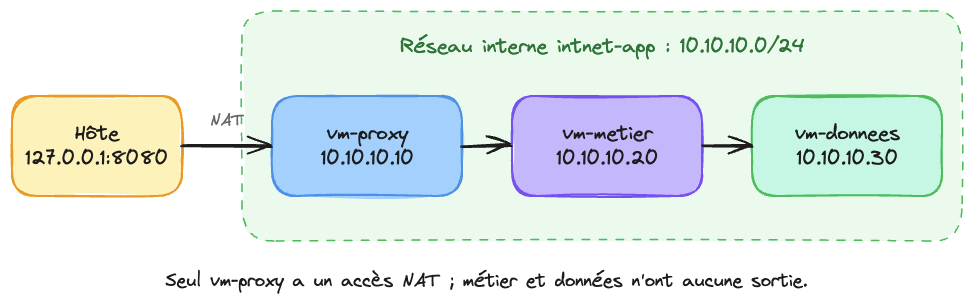
\includegraphics[width=.92\linewidth,height=3.3cm,keepaspectratio]{images/figure-3.png}
\captionof{figure}{Réseau des trois VM et point d'entrée depuis l'hôte.}\label{fig:3}
\end{minipage}\end{center}
\subsection{Installer sans accès à Internet}
Pour installer PostgreSQL et les dépendances Python sur les VM isolées, nous avons ajouté temporairement un adaptateur NAT, puis l'avons retiré avant les vérifications. Seul le proxy conserve cet accès dans la configuration finale. La même manipulation sera nécessaire lors des mises à jour.

\subsection{Déploiement des trois couches}
\begin{itemize}
\item Données : PostgreSQL écoute sur 10.10.10.30. Les règles SCRAM de pg\_hba.conf et le pare-feu nftables limitent l'accès à la VM métier. Le compte applicatif n'est pas superutilisateur.
\item Métier : Django écoute sur 10.10.10.20:8000 via Gunicorn, lancé par systemd avec un compte dédié. La configuration est dans un fichier d'environnement privé, hors du dépôt. Les migrations et la commande manage.py check ont réussi.
\item Proxy : Nginx sert le build React et les statiques, et relaie l'API.
\end{itemize}
\subsection{Vérification de l'isolation}
Nous avons testé l'isolation avec tous les services démarrés : l'hôte atteint le proxy sur le port 8080, mais ni le métier ni la base. Le proxy ne joint pas la base non plus. Un refus ne peut donc pas être attribué à un service arrêté.

La VM proxy s'est bloquée au démarrage avec la paravirtualisation KVM (catalogue inaccessible après 240 s). Le mode \og minimal\fg{} a résolu le problème. L'incident est documenté par une capture ; sa cause exacte reste inconnue.

\clearpage
\section{Déploiement en conteneurs}
\subsection{Images et composition}
Nous avons utilisé Docker Engine 28.3.3 en mode rootless, Compose 2.39.4 et le stockage fuse-overlayfs. Le démon fonctionne donc sans les privilèges root. La pile contient trois services :

\begin{itemize}
\item Métier : une image de moins de 389 Mo, avec des versions de dépendances fixées. Les dépendances sont installées avant le code pour réutiliser le cache ; Git, uv et les caches sont absents de l'image finale.
\item Proxy : Nginx avec le build React. Taille inférieure à 56 Mo.
\item Données : image officielle PostgreSQL 16, données sur un volume nommé ; les scripts d'initialisation ne s'exécutent que sur un volume vide.
\end{itemize}
Comme le montre la figure~\ref{fig:4}, compose.yaml définit deux réseaux : le frontal relie le proxy au métier ; le réseau internal: true relie le métier à PostgreSQL. Seul le proxy publie un port. Les services attendent les sondes de santé de leurs dépendances. Django joint la base par son nom DNS, donnees.

\begin{center}\begin{minipage}{\linewidth}\centering
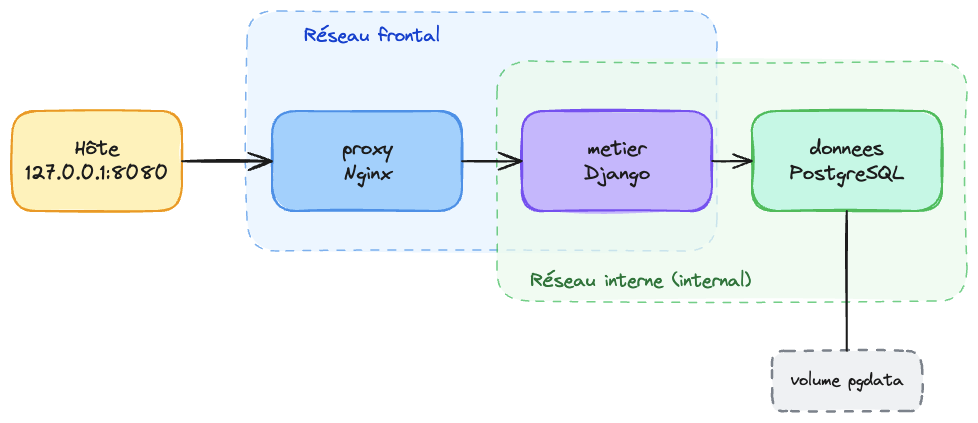
\includegraphics[width=.92\linewidth,height=4.4cm,keepaspectratio]{images/figure-4.png}
\captionof{figure}{Réseaux Docker et volume persistant de PostgreSQL.}\label{fig:4}
\end{minipage}\end{center}
\subsection{Ce que change Compose}
\begin{center}\begin{minipage}{\linewidth}\small
\captionof{table}{Mise en place manuelle et déploiement avec Compose.}\label{tab:3}
\begin{tabularx}{\linewidth}{YYY}
\toprule
\textbf{} & \textbf{Machines virtuelles} & \textbf{Conteneurs} \\
\midrule
Fichiers déclaratifs & 109 lignes de configuration (Netplan, PostgreSQL, nftables, systemd, Nginx) & 136 lignes (compose.yaml + deux Dockerfiles) \\
Procédure écrite & 183 lignes de commandes à exécuter dans l'ordre & Le fichier de composition est la procédure : docker compose up \\
Ce qui reste implicite & L'ordre des opérations, l'état des paquets installés, les adaptateurs réseau réglés dans VirtualBox & Le cache de construction, l'état du volume (déjà initialisé ou non), le moteur Docker lui-même \\
\bottomrule
\end{tabularx}
\end{minipage}\end{center}
Le tableau~\ref{tab:3} résume la différence : avec les VM, nous rejouons les installations et les réglages ; avec Compose, nous décrivons les services et leurs liens, puis l'outil les lance. La procédure docker/PROCEDURE.md détaille les contrôles à effectuer.

\clearpage
\section{Protocole et résultats au repos}
Nous avons répété trois arrêts et démarrages complets sur le même poste. Après 30 s au repos, dix requêtes GET sont envoyées au catalogue via le proxy. Le tableau~\ref{tab:4} donne la médiane des trois séries. Le démarrage s'arrête à la première réponse HTTP 200 non vide.

\begin{center}\begin{minipage}{\linewidth}\small
\captionof{table}{Mesures au repos, médianes de trois séries.}\label{tab:4}
\begin{tabularx}{\linewidth}{YYYY}
\toprule
\textbf{Grandeur} & \textbf{3 VM} & \textbf{3 conteneurs} & \textbf{Écart Docker / VM} \\
\midrule
Démarrage jusqu'au catalogue & 20,47 s & 60,62 s & +196 \% \\
Mémoire RSS côté hôte & 1,454 Gio & 0,484 Gio & -66,7 \% \\
Disque (blocs alloués) & 10,755 Gio & 0,863 Gio & -92,0 \% \\
Latence de consultation & 62,4 ms & 120,2 ms & +92,6 \% \\
Mise en place depuis zéro & \multicolumn{3}{l}{\footnotesize Non chronométrée ; temps non reconstituable.} \\
\bottomrule
\end{tabularx}
\end{minipage}\end{center}
Sous Linux, Docker tourne directement sur l'hôte. La mémoire mesurée inclut le démon, containerd, les shims et les auxiliaires rootless de réseau et de stockage. Ces coûts sont donc bien comptés dans le résultat.

\subsection{Les écarts observés}
Dans ces essais, Docker économise environ 0,97 Gio de mémoire et 9,9 Gio de disque. En contrepartie, il démarre 40 s plus tard et répond 58 ms plus lentement au repos. Le choix dépend donc du critère que l'on privilégie.

\subsection{Comment les interpréter}
\begin{itemize}
\item La mémoire et le disque : les conteneurs partagent le noyau et certaines couches des images, alors que les VM embarquent chacune un système complet. Les snapshots des VM expliquent aussi une partie de l'écart disque.
\item Le démarrage et la latence : le stockage FUSE, le réseau rootless et l'attente des sondes de santé pourraient expliquer le surcoût côté Docker. Nous n'avons toutefois pas mesuré séparément l'effet de chacun.
\item La comparaison a ses limites : les VM ont des quotas de 1/2/2 vCPU, contrairement aux conteneurs. Les versions de Python (3.12.3 / 3.12.15) et de Nginx (1.24 / 1.28) diffèrent aussi.
\end{itemize}
\subsection{Les compromis d'isolation}
Le mode rootless réduit les privilèges, mais les conteneurs partagent toujours le noyau de l'hôte. Ils n'offrent donc pas la même séparation que des VM et restent dépendants de ce noyau. Il faut aussi sauvegarder les volumes : reconstruire une image ne restaure pas les données.

L'étude de Felter et al. (IBM Research, 2014) sert de point de comparaison sur les performances des VM et des conteneurs. Notre configuration ajoute notamment FUSE et le réseau rootless ; nos résultats ne suffisent pas à attribuer l'écart à ces seules couches.

\clearpage
\section{Tests de charge}
\subsection{Plan de test et étalonnage}
Avec JMeter 5.6.3 en ligne de commande, nous avons simulé un candidat qui se connecte puis consulte ses candidatures, avec une seconde de pause entre les consultations. Chaque utilisateur a son compte fictif. Les assertions contrôlent l'identité, la session et la candidature attendue pour éviter de compter une réponse incorrecte comme un succès.

Nous avons testé 1, 5, 10 et 20 utilisateurs : 30 s de montée, 15 s de stabilisation, puis 120 s de mesure, avec deux séries en ordre inversé. L'injecteur atteint 3 250 requêtes/s sur une ressource statique Nginx, très au-dessus des 20 consultations/s possibles avec ce scénario. Il ne semble donc pas limiter ces essais.

\subsection{Résultats}
\begin{center}\begin{minipage}{\linewidth}\small
\captionof{table}{Débit et p95 selon le nombre d'utilisateurs.}\label{tab:5}
\begin{tabularx}{\linewidth}{YYYY}
\toprule
\textbf{Utilisateurs} & \textbf{Débit VM / Docker (req/s)} & \textbf{p95 VM, séries 1 / 2 (ms)} & \textbf{p95 Docker, séries 1 / 2 (ms)} \\
\midrule
1 & 0,975 / 0,983 & 33,4 / 28,4 & 21,2 / 19,0 \\
5 & 4,871 / 4,904 & 49,0 / 27,0 & 18,0 / 19,0 \\
10 & 9,738 / 9,833 & 46,0 / 29,0 & 20,0 / 20,0 \\
20 & 19,479 / 19,642 & 44,0 / 29,0 & 20,3 / 20,0 \\
\bottomrule
\end{tabularx}
\end{minipage}\end{center}
Les courbes de débit, de p95 et de taux d'erreur sont disponibles dans le dépôt : \nolinkurl{mesure/docs/courbes/ensemble.png}.

Le tableau~\ref{tab:5} résume les mesures sous charge. Les 22 199 requêtes enregistrées, montée et connexions comprises, ne contiennent aucune erreur.

\subsection{Analyse}
À 20 utilisateurs, le débit ne diffère que de 0,83 \%. Docker obtient un p95 plus bas de 54 \%, puis de 31 \% selon la série. Ce p95 est le temps sous lequel se terminent 95 \% des requêtes. Il varie de 34 \% entre les deux séries pour les VM, contre environ 1 \% pour Docker.

La seconde de pause limite le débit : avec U utilisateurs et un temps de réponse R en secondes, on attend au plus $U/(1+R)$ requêtes/s. Quelques millisecondes changent donc peu le débit, mais restent visibles sur le p95. Le réseau VirtualBox et l'absence de quotas Docker sont des pistes d'explication, sans preuve suffisante pour conclure.

Aucun service ne sature jusqu'à 20 utilisateurs. Le métier utilise le plus de CPU : 26 à 28 \% d'un c\oe{}ur côté VM, 31 à 32 \% côté Docker. Les campagnes complémentaires détaillées ci-après étendent la charge et examinent l'effet du nombre de workers Gunicorn.

Ces essais utilisent une base fictive et un parcours de consultation. Ils ne couvrent pas les téléversements de CV, les pannes ou une utilisation en production. Le moteur Docker s'est arrêté pendant la campagne initiale ; la charge de l'hôte variait entre les séries. JMeter et le déploiement partagent le même poste physique : ils se disputent ses ressources CPU, mémoire et E/S. L'étalonnage statique contrôle une partie du chemin de mesure, mais ne supprime pas ce biais à forte charge.

\clearpage
\subsection{Mesures complémentaires de capacité}
La campagne de capacité conserve 48 essais : montée de 30 s, stabilisation de 15 s, plateau de 120 s et pause de 1 s. La charge demandée atteint 160 utilisateurs côté VM et 320 côté Docker, avec affinement des paliers. Les seuils de service sont un p95 au plus égal à 1\,000 ms et au plus 1 \% d'erreurs ; la répétabilité impose un écart maximal de 10 \% entre les séries.

\begin{center}\begin{minipage}{\linewidth}\small
\captionof{table}{Principaux paliers de capacité ; valeurs des séries 1 / 2.}\label{tab:capacity}
\begin{tabularx}{\linewidth}{>{\hsize=.80\hsize}Y >{\hsize=1.00\hsize}Y >{\hsize=1.20\hsize}Y >{\hsize=1.00\hsize}Y >{\hsize=1.00\hsize}Y}
\toprule
\textbf{Utilisateurs} & \textbf{Débit VM (req/s)} & \textbf{p95 VM (ms)} & \textbf{Débit Docker (req/s)} & \textbf{p95 Docker (ms)} \\
\midrule
80 & 77,35 / 77,27 & 74 / 75,45 & 78,64 / 78,54 & 24 / 26 \\
120 & 86,37 / 86,32 & 533,85 / 551 & 117,86 / 117,90 & 30 / 30 \\
140 & 85,10 / 85,08 & 766 / 876 & 137,04 / 137,39 & 48 / 39 \\
150 & 86,11 / 83,63 & 906,40 / 966,25 & 146,13 / 146,55 & 79 / 64 \\
160 & 84,13 / 84,56 & 1\,061 / 1\,046 & 153,19 / 154,79 & 176,90 / 102 \\
180 & -- & -- & 162,06 / 164,85 & 253 / 240 \\
190 & -- & -- & 164,12 / 163,21 & 326 / 295 \\
\bottomrule
\end{tabularx}
\end{minipage}\end{center}
Le tableau~\ref{tab:capacity} porte sur les consultations réussies pendant le plateau ; ces essais n'ont aucune erreur. Les p95 restent séparés. Les charges supérieures à la borne de refus VM ne sont pas rejouées.

Le débit VM plafonne autour de 84 à 86 req/s dès 120 utilisateurs ; le p95 dépasse 1 s à 160 dans les deux séries. Docker atteint environ 163 à 164 req/s à 190 utilisateurs. À 200, sa première série ne maintient que 8 utilisateurs actifs et compte 192 erreurs sur l'essai entier (45 connexions et 147 consultations) ; la seconde maintient 200 utilisateurs, 164,78 req/s et un p95 de 379 ms. Les tentatives à 240 et 320 n'en maintiennent que 190 et 20 : ces plateaux sont invalides et ne démontrent pas la tenue aux charges demandées.

Nous observons donc un plafonnement du débit et une hausse de latence, mais aucune capacité maximale validée. Le p95 varie de 13,40 \% à 140 utilisateurs côté VM et jusqu'à 53,71 \% à 160 côté Docker ; l'interruption documentée et les essais incomplets limitent aussi l'interprétation.

\subsection{Courbe de montée en charge}
\begin{center}\begin{minipage}{\linewidth}\centering
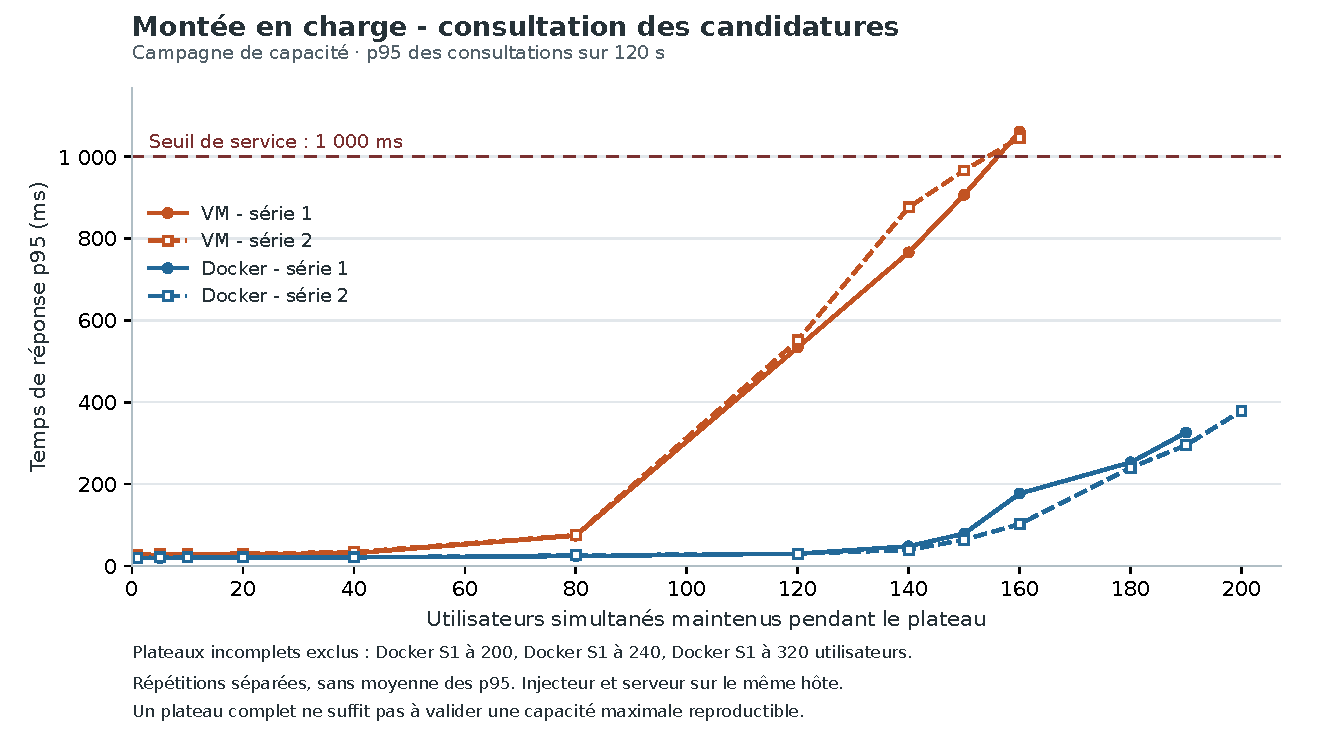
\includegraphics[width=\linewidth]{../mesure/docs/courbes/capacity-p95.pdf}
\captionof{figure}{Temps de réponse en fonction des utilisateurs simultanés. Les 45 points correspondent aux plateaux complets de la campagne de capacité ; les deux séries restent distinctes.}\label{fig:capacity}
\end{minipage}\end{center}
La figure~\ref{fig:capacity} utilise les paliers réellement mesurés de cette campagne, sans ajouter de valeurs intermédiaires ni moyenner les p95. En VM, les deux séries dépassent le seuil de 1\,000 ms à 160 utilisateurs. Le point Docker à 200 n'existe qu'en série 2 ; les plateaux incomplets de la série 1 à 200, 240 et 320 sont exclus. La tenue d'un plateau ne suffit pas à établir une capacité maximale reproductible, notamment lorsque l'injecteur et le serveur partagent le même hôte.

La figure, le CSV de ses sources et le script de régénération sont liés dans la \href{https://github.com/OmarBenje/Intern/blob/master/mesure/docs/capacity-summary.md}{synthèse des mesures complémentaires}. Les essais à faible charge historiques et ceux comparant les workers constituent des campagnes distinctes.

\subsection{Effet du nombre de workers Gunicorn}
Deux campagnes comparent 2 et 4 workers, dans l'ordre 2/4 puis 4/2, avec les mêmes données restaurées et les mêmes ressources pour chaque déploiement. Elles couvrent 80, 100 et 130 utilisateurs en VM, puis 150, 180 et 200 sous Docker. Le tableau~\ref{tab:workers} présente le dernier palier de chaque campagne.

\begin{center}\begin{minipage}{\linewidth}\small
\captionof{table}{Comparaison des workers ; valeurs des séries 1 / 2, zéro erreur.}\label{tab:workers}
\begin{tabularx}{\linewidth}{YYYYY}
\toprule
\textbf{Déploiement et charge} & \textbf{Débit, 2 workers (req/s)} & \textbf{Débit, 4 workers (req/s)} & \textbf{p95, 2 workers (ms)} & \textbf{p95, 4 workers (ms)} \\
\midrule
VM, 130 & 86,28 / 84,24 & 96,63 / 99,78 & 708 / 721 & 521 / 443 \\
Docker, 200 & 163,47 / 162,14 & 195,19 / 195,19 & 373 / 385 & 60 / 55 \\
\bottomrule
\end{tabularx}
\end{minipage}\end{center}
À 200 utilisateurs sous Docker, 4 workers améliorent le débit de 19,4 \% puis 20,4 \% et réduisent le p95. Cela soutient l'hypothèse d'une limite liée au nombre de workers. Les p95 VM ne satisfont pas le critère strict de répétabilité : le gain observé ne valide pas une capacité maximale. Les synthèses et protocoles des trois campagnes sont dans \nolinkurl{mesure/preuves/README.md}.

\clearpage
\section{Bilan}
\subsection{Ce que le projet montre}
\begin{itemize}
\item Les VM nous ont donné une isolation plus forte et, dans cette configuration, un démarrage plus rapide. Elles utilisent cependant environ trois fois plus de mémoire et douze fois plus de disque.
\item Docker réduit les ressources utilisées et simplifie la reconstruction de la pile avec Compose. En revanche, le noyau est partagé et le mode d'exécution influence les performances.
\item Jusqu'à 20 utilisateurs, les débits sont proches. Les campagnes à forte charge montrent ensuite un plafonnement et l'intérêt de comparer les réglages de Gunicorn, sans établir de capacité maximale reproductible.
\item Nous avons pu déployer le même code dans les deux environnements grâce à la configuration externalisée et à la séparation des couches. La comparaison de l'interface avec le prototype Figma est réalisée (T25).
\end{itemize}
\subsection{Limites et suites}
\begin{itemize}
\item Refaire les tests sur deux machines physiques distinctes : une machine cliente dédiée à JMeter génère les requêtes ; une seconde héberge le serveur testé, VM ou conteneurs. Cette séparation évite la concurrence directe entre injecteur et serveur pour les ressources du même hôte. Mesurer aussi le réseau et l'injecteur, stabiliser l'hôte serveur et répéter sans interruption.
\item Aligner les quotas CPU et mémoire, puis comparer les modes Docker classique et rootless en contrôlant aussi le stockage.
\item Chronométrer la mise en place depuis zéro des deux déploiements.
\item Étudier un répartiteur de charge (\textit{load balancer}) devant plusieurs instances de l'API Django et Gunicorn, avec des sondes de santé. Partager les sessions via PostgreSQL et les fichiers via le stockage commun, puis vérifier la tenue des connexions à la base.
\item Comparer une instance et plusieurs instances avec ce répartiteur, mesurer débit, p95 et erreurs, puis tester la perte d'une instance. Cette architecture est une perspective : elle n'a pas été déployée ni mesurée dans ce projet.
\end{itemize}
\subsection*{Références}
\begin{itemize}
\item W. Felter, A. Ferreira, R. Rajamony, J. Rubio, An Updated Performance Comparison of Virtual Machines and Linux Containers, IBM Research, 2014.
\item Documentation Docker : \url{https://docs.docker.com/engine/security/rootless/}.
\item Documentation Cloudflare R2 : \url{https://developers.cloudflare.com/r2/examples/aws/boto3/}.
\item Preuves brutes du projet : deploiement/docs/, docker/docs/, mesure/preuves/ (dépôt GitHub Intern).
\end{itemize}
\end{document}
